% !TeX encoding = UTF-8
% !TeX spellcheck = pl_PL

\PassOptionsToPackage{breaklinks}{hyperref}
\PassOptionsToPackage{svgnames}{xcolor}

\documentclass[polish, 12pt, aspectratio=169]{beamer}

\usepackage[nosingleletter, lastparline]{impnattypo}
\usepackage[polish]{babel}
\usepackage{minted}
\usepackage{csquotes}
\usepackage[backref, backend=bibtex]{biblatex}
\usepackage{bookmark}
\usepackage{hyperref}
\usepackage[babel, tracking]{microtype}
\usepackage{booktabs}
\usepackage{graphicx}
\usepackage{parskip}
\usepackage{framed}
\usepackage{tabularx}
\usepackage{ltablex}
\usepackage{adjustbox}
\usepackage{float}
\usepackage{longtable}
\usepackage{subcaption}
\usepackage[strings]{underscore}
\usepackage{tikz}
\usepackage{amsmath}
\usepackage{amssymb}
\usepackage{xfrac,unicode-math}
\usepackage{bm}
\usepackage{physics}

\usetheme[progressbar=frametitle]{metropolis}
\setmonofont{JetBrainsMono}[
    Scale=0.8,
    Extension=.ttf,
    UprightFont=*-Regular,
    BoldFont=*-Bold,
    ItalicFont=*-Italic,
    BoldItalicFont=*-BoldItalic
]

\title{Transformacja Fouriera}
\author{Piotr Rogulski}
\date{\today}

\addbibresource{fourier.bib}

\setbeamertemplate{frametitle continuation}[from second][]

\begin{document}

\frame{\titlepage}

\begin{frame}{Agenda}
    \setbeamertemplate{section in toc}[sections numbered]
    \tableofcontents
\end{frame}

\section{Transformacja Fouriera}

\begin{frame}{Joseph Fourier (1768--1830)}
    \begin{columns}
    \column{0.7\linewidth}
        \begin{itemize}[<+->]
            \setlength\itemsep{1em}
            \item francuski matematyk i fizyk
            \item badania wymiany ciepła (\enquote{Théorie analytique de la chaleur}, 1822)
            \item rozkład funkcji okresowej na szereg trygonometryczny --- \textbf{szereg Fouriera}
        \end{itemize}
    \column{0.25\linewidth}
        \begin{figure}
            \includegraphics<3>[width=\linewidth]{img/fourier-series.eps}
        \end{figure}
    \end{columns}
\end{frame}

\begin{frame}{Transformacja Fouriera}
    \pause{}
    \begin{itemize}[<+->]
        \item operator liniowy
        \item przekształca funkcję rzeczywistą na funkcję rzeczywistą \\
              \( \mathcal{F}: (\mathbb{R}^n \to \mathbb{R}^n) \to (\mathbb{R}^n \to \mathbb{R}^n) \)
        \item przekształca funkcję w dziedzinie czasu na funkcję w dziedzinie częstotliwości
    \end{itemize}
\end{frame}

\begin{frame}{Transformacja Fouriera}
    \Huge
    \begin{equation*}
        \mathcal{F}(f)(\xi) = \int_{-\infty}^{\infty} f(x) e^{-2\pi i x \xi} dx
    \end{equation*}
    \pause{}
    \small
    W postaci n-wymiarowej:
    \normalsize
    \vspace{-1em}
    \begin{equation*}
        \mathcal{F}(f)(\symbf{\xi}) = \int_{\mathbb{R}^n} f(\symbf{x}) e^{-2\pi i (\symbf{x \cdot \xi})} d\symbf{x}
    \end{equation*}
\end{frame}

\begin{frame}{Własności transformaty Fouriera}
    \begin{itemize}
        \setlength\itemsep{0.5em}
        \item<2-> liniowość: \( \mathcal{F}(af + bg) = a\mathcal{F}f + b\mathcal{F}g \)
        \item<3-> przesunięcie: \( \mathcal{F}(f(x - a)) = e^{-2\pi i a \xi} \mathcal{F}f(\xi) \)
        \item<3-> modulacja: \( \mathcal{F}(e^{2\pi i a x} f(x)) = \mathcal{F}f(\xi - a) \)
        \item<4-> symetria: \( \mathcal{F}(\mathcal{F}f)(x) = f(-x) \)
        \item<5-> konwolucja: \( \mathcal{F}(f * g) = \mathcal{F}f \cdot \mathcal{F}g \)
        \item<6-> pochodna: \( \mathcal{F}(f') = 2\pi i \xi \mathcal{F}f \)
    \end{itemize}
\end{frame}

\section[DFT \\ {\normalsize Discrete Fourier Transform}]{DFT}

\begin{frame}{Dyskretna transformacja Fouriera}
    \begin{itemize}
        \item transformacja Fouriera dla funkcji dyskretnych
    \end{itemize}
\end{frame}

\begin{frame}{Dyskretna transformacja Fouriera}
    \Huge
    \begin{equation*}
        X_k = \sum_{n=0}^{N-1} x_n e^{-2\pi i \frac{kn}{N}}
    \end{equation*}
    \pause{}
    \small
    W postaci n-wymiarowej:
    \normalsize
    \vspace{-1em}
    \begin{equation*}
        X_{\symbf{k}} = \sum_{\symbf{n} = \symbf{0}}^{\symbf{N} - \symbf{1}} x_{\symbf{n}} e^{-2\pi i \frac{\symbf{k \cdot n}}{\symbf{N}}}
    \end{equation*}
\end{frame}

\begin{frame}{Macierz DFT}
    \begin{itemize}[<+->]
        \item \( X_k = \sum_{n=0}^{N-1} x_n e^{-2\pi i \frac{kn}{N}} \Longleftrightarrow X = Wx\), gdzie \( W_{kn} = e^{-2\pi i kn / N} \)
        \item Elementy \(W\) są postaci \( w_{kn} = \omega^{kn} \), gdzie \( \omega = e^{-2\pi i / N} \)
        \item \(W = \frac{1}{N} \begin{bmatrix}
            1 & 1 & 1 & \cdots & 1 \\
            1 & \omega & \omega^2 & \cdots & \omega^{N-1} \\
            1 & \omega^2 & \omega^4 & \cdots & \omega^{2(N-1)} \\
            \vdots & \vdots & \vdots & \ddots & \vdots \\
            1 & \omega^{N-1} & \omega^{2(N-1)} & \cdots & \omega^{(N-1)(N-1)}
        \end{bmatrix}\)
        \item \(W\) jest macierzą Vandermonde'a dla pierwiastka z jedności: \(\omega^N = 1\)
    \end{itemize}
\end{frame}

\section[FFT \\ {\normalsize Fast Fourier Transform}]{FFT}

\begin{frame}{Dlaczego FFT?}
    \begin{itemize}
        \item potrzeba szybkiego obliczania DFT
        \item złożoność obliczeniowa DFT\@: \( O(N^2) \)
        \item<2|alert@2> złożoność obliczeniowa FFT\@: \( O(N \log N) \)
    \end{itemize}
\end{frame}

\begin{frame}{Algorytm Cooleya-Tukeya (1965)}
    \begin{columns}
    \column{0.5\linewidth}
        \begin{itemize}
            \setlength\itemsep{1em}
            \item dziel i zwyciężaj
            \item oblicza DTF rozmiaru \( N = N_1 N_2 \) za pomocą DFT rozmiaru \( N_1 \) i \( N_2 \)
            \item osiąga złożoność \( O(N \log N) \) dla liczb \enquote{gładkich}
        \end{itemize}
    \pause{}
    \column{0.5\linewidth}
        \vspace{1em}
        \begin{figure}
            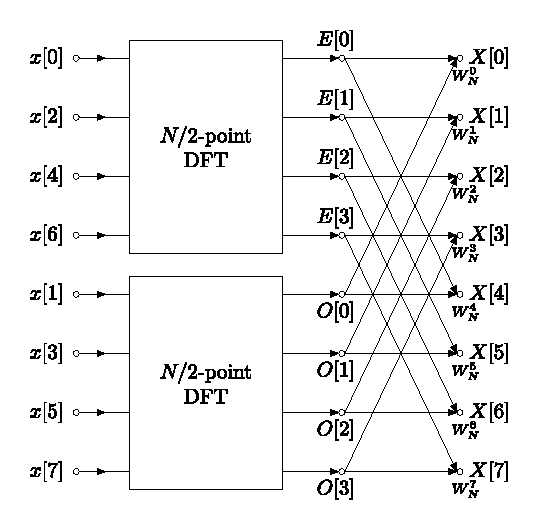
\includegraphics[width=0.9\linewidth]{img/fft-diagram.eps}
            \caption*{FFT dla decymacji Radix-2}
        \end{figure}
    \end{columns}
\end{frame}

\setbeamercovered{transparent}

\begin{frame}{Inne algorytmy FFT}
    \begin{columns}
    \column{0.5\linewidth}
        \begin{itemize}[<+>]
            \setlength\itemsep{1em}
            \item algorytm Bluesteina --- Chirp Z-transform
            \item algorytm Radera
            \item Hexagonal fast Fourier transform
        \end{itemize}
    \column{0.5\linewidth}
        \vspace{1em}
        \begin{figure}
            \begin{overprint}
                \includegraphics<1>[width=\linewidth]{img/chirp-z.png}
                \includegraphics<2>[width=\linewidth]{img/rader.jpg}
                \includegraphics<3>[width=\linewidth]{img/hex.jpg}
            \end{overprint}
        \end{figure}
    \end{columns}
\end{frame}

\setbeamercovered{invisible}

\section{Zastosowania transformacji Fouriera}

\begin{frame}{Spektroskopia fourierowska}
    \vspace{0.05\textheight}
    \begin{figure}
        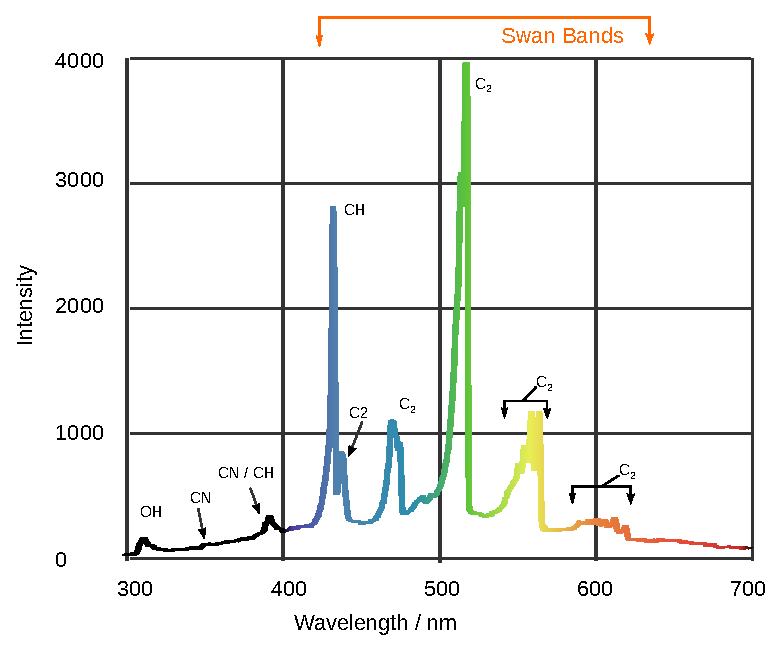
\includegraphics[
            width=\linewidth,
            height=0.75\textheight,
            keepaspectratio,
        ]{img/spectrum.eps}
        \caption*{Spektrum emisyjne płomienia palnika butanowego}
    \end{figure}
\end{frame}

\begin{frame}{FTIR}
    \vspace{0.5em}
    \begin{columns}
    \column{0.45\linewidth}
        \begin{figure}
            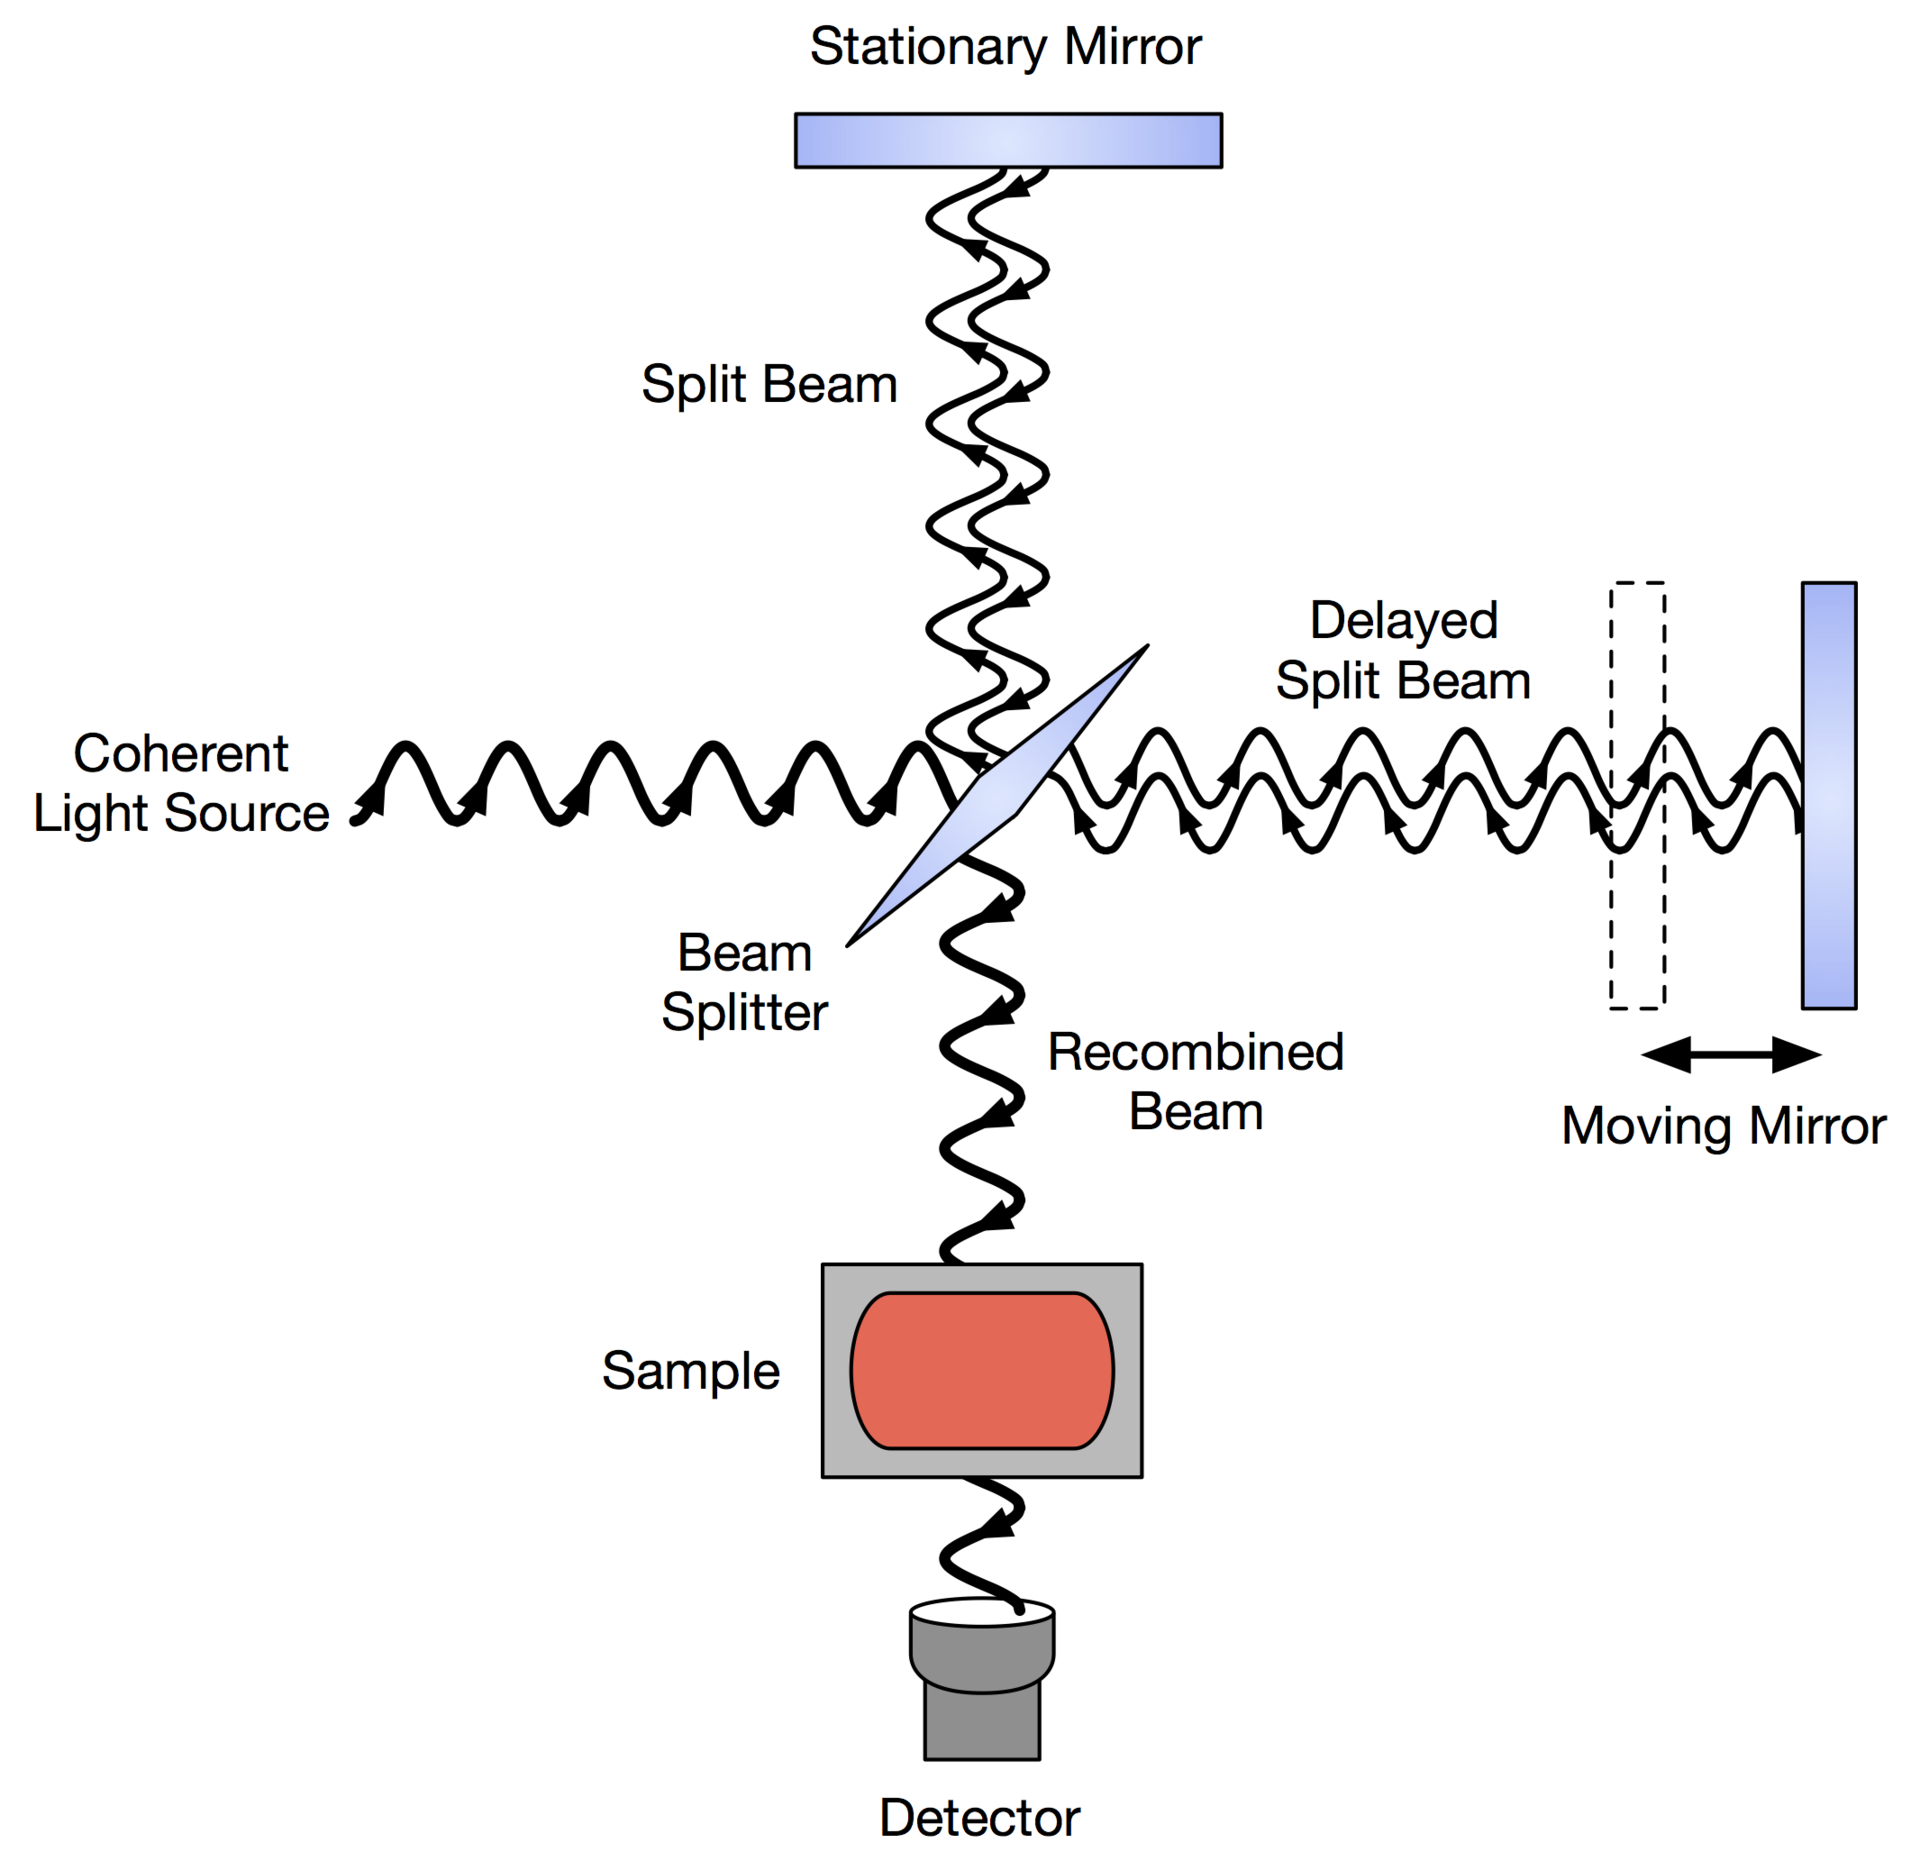
\includegraphics[width=\linewidth]{img/interferometer.png}
            \caption*{Interferometr}
        \end{figure}
    \pause{}
    \column{0.45\linewidth}
        \begin{figure}
            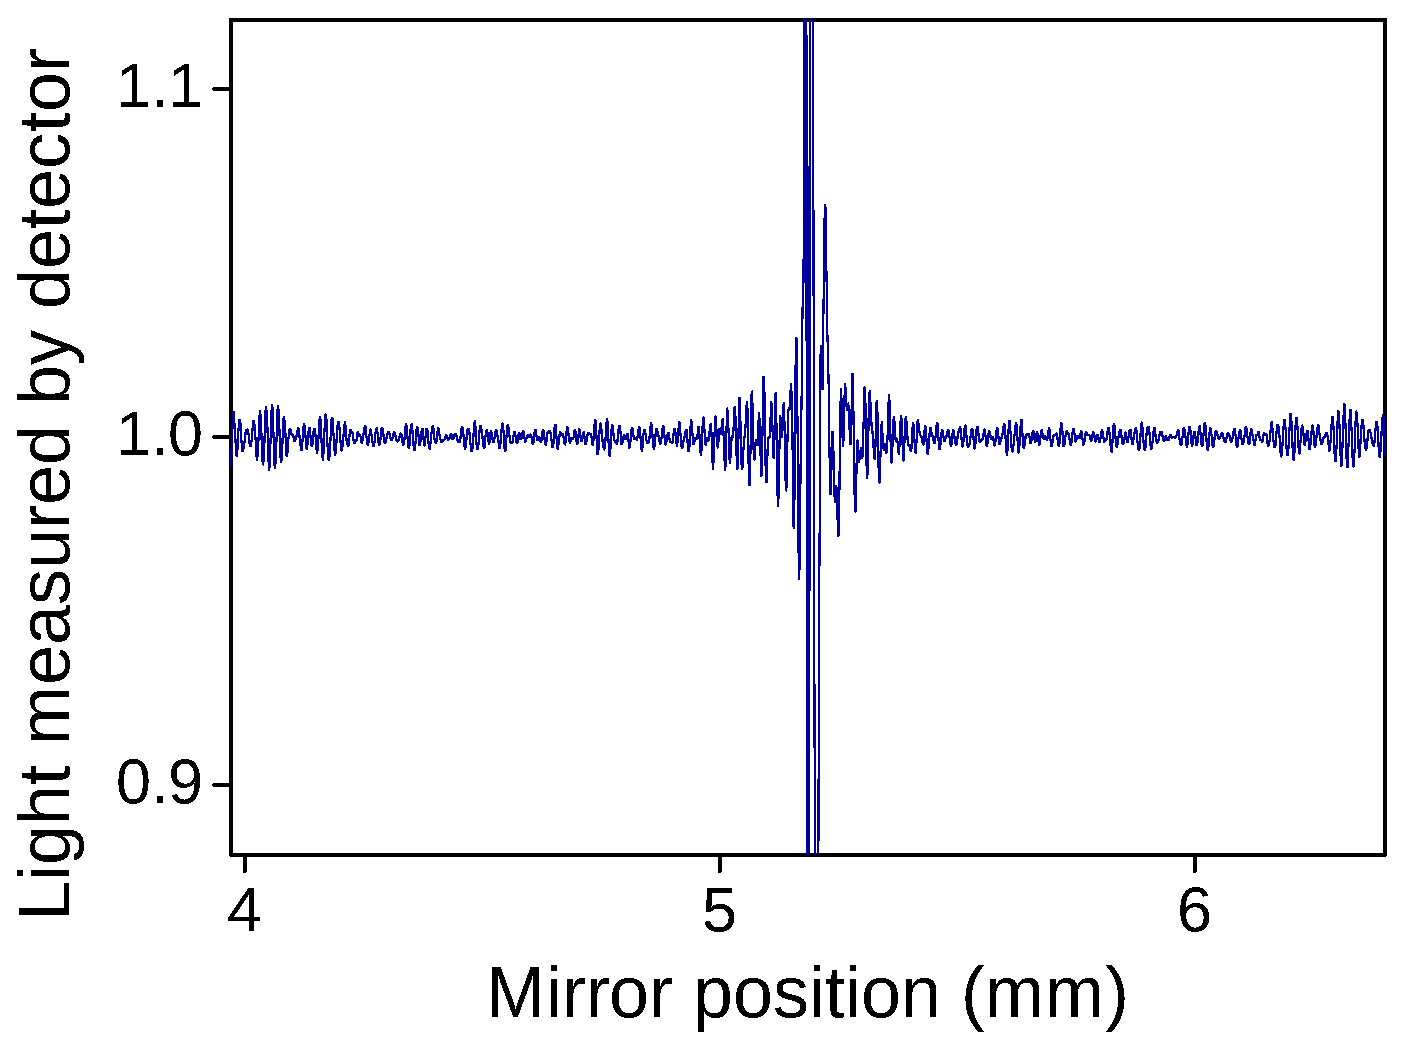
\includegraphics[width=\linewidth]{img/ftir.eps}
            \caption*{Interferogram}
        \end{figure}
    \end{columns}
\end{frame}

\begin{frame}{Analiza równań różniczkowych}
    \pause
    \begin{itemize}[<+->]
        \item Transformacja Fouriera pozwala uprościć rozwiązywanie równań różniczkowych
        \item Przykład: oscylator harmoniczny: \( \dv[2]{x}{t} + 2\gamma \dv{x}{t} + \omega_0^2 x(t) = \frac{f(t)}{m} \)
        \item Po transformacji obu stron: \( -\omega^2 X(\omega) - 2i\gamma\omega X(\omega) + \omega_0^2 X(\omega) = \frac{F(\omega)}{m} \) \\
              gdzie \( X(\omega) = \mathcal{F}(x(t)) \) i \( F(\omega) = \mathcal{F}(f(t)) \)
        \item Jest to równanie algebraiczne: \( X(\omega) = \frac{F(\omega)}{m(\omega_0^2 - \omega^2 - 2i\gamma\omega)} \)
        \item Aby otrzymać rozwiązanie w dziedzinie czasu, należy obliczyć odwrotną transformatę Fouriera
        \item \( x(t) = \frac{1}{2\pi} \int_{-\infty}^{\infty} X(\omega) e^{i\omega t} d\omega \)
    \end{itemize}
\end{frame}

\begin{frame}{Discrete cosine transform}
    \begin{columns}
    \column{0.5\linewidth}
        \begin{itemize}[<+->]
            \setlength\itemsep{1em}
            \item dyskretna transformacja kosinusowa
            \item podobna do DFT, ale wykorzystuje tylko liczby rzeczywiste
            \item stosowana w kompresji JPEG, MPEG, MP3
        \end{itemize}
    \pause{}
    \column{0.45\linewidth}
        \vspace{1em}
        \begin{figure}
            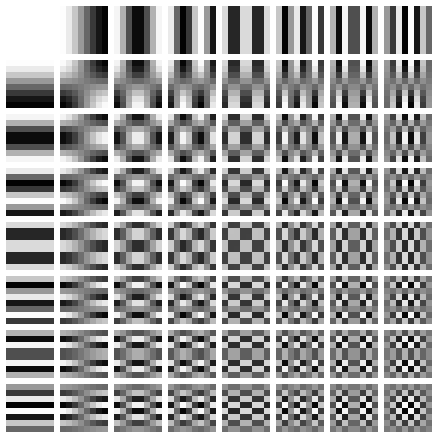
\includegraphics[width=\linewidth]{img/dct-jpeg.png}
            \caption*{Częstotliwości DCT dla obrazu JPEG}
        \end{figure}
    \end{columns}
\end{frame}

\section*{Bibliografia}

\begin{frame}[allowframebreaks]{Bibliografia}
    \nocite{*}
    \printbibliography[heading=none]
\end{frame}

\end{document}
